%*******************************************
\section{Initial User Survey}
%*******************************************
\label{s:survey}
Before elaborating on the app design we ran an initial survey, to gain some input, of which we illustrate the main objectives in this chapter.
 Furthermore, it provides details regarding the contents of the survey.
Finally, this chapter presents the results, evaluates the questionnaire and discusses how the answers influenced our further app elaborations.
 To the best of our knowledge there do not exist other surveys which resemble ours and additionally were conducted in Germany.

%============================================
\subsection{Main Objectives}
%============================================
Our main objectives of this survey were twofold:

\begin{enumerate}
	\item \textit{Awareness and Knowledge:} One goal of the survey was to comprehend what exactly Internet users understand under phishing.
 With a Likert scale we furthermore aspired to figure out how they assess their knowledge on Internet security.

	\item \textit{Preferences of Users:} Another purpose of the survey was to get an idea of the users' preferences with regard to an educational app.
 For example, they were asked whether they found a quiz based approach reasonable for learning purposes.

\end{enumerate}
%============================================
\subsection{Survey Details}
%============================================
This section provides details about our questionnaire, how we distributed it and how we filtered the surveys in order to consider our target group for the results and evaluation.
The complete survey form can be consulted in \autoref{s:presurvey_form}.

\subsubsection{Questionnaire}
In the following we present the structure of our questionnaire and what we intended to achieve with each section of it.
 
\begin{enumerate}
	\item \textit{General Information:} In this section the participant is asked to provide information regarding his gender, age, his professional qualification as well as his field of study or work.
 The main purpose of this section is to exclude participants which do not fit into our target group.

	\item \textit{Internet Usage:} Here, the participant is asked how often he uses the Internet, whether he owns a smartphone and which applications he uses on his desktop computer and which ones he uses on his smartphone.
 This section is intended to give us an overview of the user's Internet usage and helps us exclude participants who do not fit into our target group.

	\item \textit{Self-Assessment:} In this part of the survey, the participant has to indicate how much he agrees with the presented statements with the aid of a Likert scale.
 The statements mainly refer to their self-assessment regarding their knowledge about Internet security.
 For example, they have to assess, whether they think they have enough knowledge to avoid the dangers of the Internet or whether they think it is easy for them to distinguish legitimate e-mails from fake ones.
 This section is partially based on Likert scale statements used by DIVSI~\cite{divsi2012divsi}.
	\item \textit{Phishing:} Here, the participant gets questions to the topic of phishing.
 In particular, he is asked which services and which user information are endangered by phishing attacks.
 This section purposes to find out what the participants know and think about phishing.

	\item \textit{Anti-Phishing App:} This section asks the user for his preferences regarding an anti-phishing education app.
 With the aid of a Likert scale he is requested to assess, for example, whether he likes the idea of a game with a fish, whether he finds text based education appropriate, or whether he would have fun with a question-answer (quiz) game.

	\item \textit{Further Survey Progress:} In this part of the survey the user can provide his e-mail address in case he wants to get information about the further progress of the survey or in case he would like to test the app.

\end{enumerate}

\subsubsection{Distribution}
In total 251 persons participated in our survey.
 We set up an online survey as well as asked students to fill out our printed survey.
 In the following we briefly explain our distribution process.


\begin{description}[leftmargin=0cm]
	\item[Printed Survey:] To reach participants for our printed survey we contacted multiple professors and asked them whether we could have 10 minutes of their lecture time to have their students filled out our printed survey.
 Moreover, we asked our friends and relatives whether they can ask their friends, colleagues or customers to fill out the questionnaire.

	\item[Online Survey:] The online survey was mainly distributed digitally.
 We contacted our friends and asked them to participate in the survey.
 We also demanded to forward the link to their friends to reach a wide range of people.

\end{description}

\subsubsection{Select Targeted Participants for Evaluation}

\autoref{table:prestudy_filter} summarizes what kind of answers we used in order to exclude participants from the survey who do not fit into our target group.
\begin{table}[hHtbp]
\centering
    \begin{tabular}{ | p{4.5cm} | p{10cm} |}
    \hline\textbf{Question} & \textbf{Filtering}  \\  \hline
		\hline\  Age & We consider all adults ranging from 18 - 65 years.
 \\
    \hline\  Gender & We do not exclude any gender.
 \\ 
    \hline\  Professional qualification & The participant does not have to exhibit a specific professional qualification to be considered for the results and evaluation.
 \\ 
		\hline\  Field of study/work & Students, employees or employers in the field of computer science or electrical engineering are ruled out as they do not belong to our target group (cf. Attackability in \autoref{s:target_group_def}).
 \\ 
	  \hline\ Frequency of Internet usage & Participants who have indicated ``rarely'' as the answer to this question do not belong to our target group and thus are filtered out (cf. Attackability in \autoref{s:target_group_def}).
 \\ 
	  \hline\ Used Internet applications  &  The listed applications include, for example, browser, e-mail, shopping as well as banking.
 Any service of the Internet is potentially endangered by phishing.
 For this reason we do not use this question to sort out participants (cf. Attackability in \autoref{s:target_group_def}).
\\ 
    \hline\ Owning a smartphone  & With the app we particularly target Android smartphone owners since only those can use our final app on a regular basis (cf. Android Users in \autoref{s:target_group_def}).
 Yet, for this particular study we consider it sufficient to own any kind of smartphone.
Therefore, participants who do not have a smartphone are ruled out.
 \\
		\hline\ Used smartphone applications in the Internet  & The listed applications include, for example, browser, e-mail, shopping as well as banking.
 Any service of the Internet is potentially endangered by phishing.
 For this reason we do not use this question to exclude participants.
 \\
    \hline\ Number of received commercial e-mails per week  & We do not sort out out any participants with this question.
 \\
    \hline\ Number of received e-mails asking for personal data  & We do not sort out any participant with this question.
 \\
    \hline\ User reads up on topics related to dangers in the Internet  &  Participants who have chosen ``no'' as their answer are filtered out.
 We specifically target users who are interested in getting safer on the Internet (cf. Motivation in \autoref{s:target_group_def}).
 As the participants, who have indicated ``no'', do not seem to have any interest in this, they will most likely do not show interest for our app.
This is why we regard them as not belonging to our target group and exclude them from the analysis and evaluation.
\\
    \hline\  Section to self-assessment regaring their knowledge about Internet security &  We do not sort out participants based on their selection in this section.
\\
		\hline\  Section to questions related to phishing itself & We do not sort out participants based on their selection in this section.
 \\
    \hline\  Section to preferences for an anti-phishing education app & We do not sort out participants based on their selection in this section.
\\
    \hline
    \end{tabular}
    \caption{Filtering rules for the phishing survey}
    \label{table:prestudy_filter}
    
\end{table}

In the succeeding section we present and evaluate the results of the study.
 With the filtering we had 169 remaining participants matching our target group.
These participants were considered for the evaluation.

%============================================
\subsection{Results and Evaluation}
%============================================
\label{s:survey_results}
The study yielded interesting results which should be considered when designing an anti-phishing education app, either for this as well as for future work.
 This section outlines the results of the study.


\begin{description}[leftmargin=0cm]
	\item[General Information:] The gender ratio of our survey participants was more or less balanced.
 40.83\% of the users were female and 56.80\% of them were male.
 The remaining 2.37\% did not indicate any gender.
 The average age of our participants was 27.59, the youngest participants were 19 years old, the oldest were 63 years old.
 Most of the survey participators, 48.52\%, obtained a university degree.
 24.85\% of them did not have any professional qualification (yet). 17.75\% did an apprenticeship and the remaining participants had a master craftsman certificate or did not indicate any professional qualification in the survey.
	
	\item[High Rate of Android Users:] The majority of the participants were Android users.
 In total about 60\% of the study participants used an Android smartphone.
 The remaining 40\% were iOS users.
 This result roughly relates to the general market share for these platforms and additionally supports our decision for the implementation of an Android application (cf. \autoref{s:sys_requirements}).

	\item[High Internet Usage Frequency:] 51.48\% of the users indicated that they were online several times a day.
 Another 30.18\% indicated that they were online even constantly.
 As a consequence, over 80\% of the survey participants are frequently online.
 This is depicted in \autoref{fig:internet_usage}. Being online is always related with being attackable and vulnerable to dangers of the Internet, such as phishing attacks (cf. Attackability in \autoref{s:target_group_def}), while the extent of the vulnerability of course also depends on other factors, such as the expertise of the person being online.
	
	\item[Usage Distribution of Internet Applications:] \autoref{fig:desktop_apps} and \autoref{fig:smartphone_apps} summarize the usage distribution of Internet applications on a desktop computer and on smartphones.
 Almost all participants, 99.41\%, make use of e-mails on their desktop computer.
 88.76\% of the smartphone owners use their e-mail application on the smartphone, which is still a high percentage.
 As we previously mentioned in \autoref{s:attack_channels}, e-mail is a common attack channel for phishing attempts.
 Consequently, all users of e-mail applications, including webmail, are potentially endangered by phishing attacks.
 The same threat of phishing applies to participants using browsers for surfing.
% A common way to trick users to disclose their confidential information is the use of fake websites.
% These websites can be reached by clicking on a link in an e-mail, SMS, in online social network, or instant messaging systems as well as by simply surfing on the Internet.
 About 80\% of all considered participants make use of desktop or smartphone browsers.
 Furthermore, it is conspicuous that banking is far less used on smartphones compared to desktop computers.
 While about 74.56\% of the participants make use of online banking on the desktop computer, only 26.63\% use it on their smartphones, which is still a quarter of the participants.
	The question to ask here is if these users utilize the browser for online banking or if they use dedicated apps provided by their bank which would be safer.
 Whether these users make use of apps or apply their online banking with a regular browser, they might be more likely to react to phishing e-mails on their smartphone, which claim to come from their bank, compared to other users who manage their financial arrangements on a desktop computer and thus are less likely to access a phishing website over their smartphone (cf. \autoref{s:antiphishing_on_smartphone}). To sum it up, all the listed categories of applications are used by the participants, on their smartphones as well as on their desktop computers.
 For this reason, we decided to use a broad range of URL examples of different website categories for the final app.
 For future research, one could consider to put the main focus on URLs from specific categories which are mainly targeted by phishing attacks and depend on the usage distribution.

	\item[Self-Assessment - Knowledge to avoid dangers of Internet:] 18.34\% of the participants strongly agree that they have enough knowledge to avoid the dangers of the Internet. Further 45.56\% agree with the statement and only about 13\% disagree or strongly disagree with this statement.
 As a consequence the majority of the participants are quite confident that they can avoid the security related risks raised by the Internet.
The general question to ask in these self-assessing statements is how well they reflect the reality.
In this case it is questionable whether 63.9\% of the participants are in fact capable of protecting themselves against the threats of the Internet.
	
	\item[Self-Assessment - Distinguish legitimate from illegitimate e-mails:] 87.23\% of the participants think that they can easily distinguish legitimate e-mails from fake ones (they agree or strongly agree).
 Only about 8\% of the participants did not agree or strongly disagreed with this statement.
 This arouses the suspicion that the users are not aware of how easy it is to spoof the ``from field'' of an e-mail, or to create credible message contents which in fact may persuade the receiver that the e-mail is trustworthy.
Therefore, we believe that the user should be made aware of this misconception.
For this reason, the part of the app which is supposed to increase a user's security awareness addresses this issue (cf. \autoref{s:app_design}).
	
	\item[Self-Assessment - Trust in e-mails from known parties:] The majority of the participants trust e-mails which come from persons they know.
 Approximately 20\% strongly agreed and 57\% agreed with this statement.
 Only about 2\% strongly disagreed and about 5\% of the participants disagreed with this statement.
 This again shows that most of the participants are not aware that spoofing the ``from field'' of an e-mail is easy to achieve.
 These users are likely to react to e-mails which claim to be, for example, from friends.
 Such e-mails may actually contain links to the download of malware or malicious websites.
We address the misconception of believing that e-mails can be trusted, whether they are received from friends or other trusted parties, with our awareness part of the app (cf. \autoref{s:app_design}).


	\item[Self-Assessment - Internet security is only related to financial applications:] The answers to this statement showed that the majority of the participants are aware that security related issues on the Internet do not solely concern financial applications.
 49.7\% of the users strongly disagreed with this statement and another 24.26\% disagreed.
 Only about 10\% of the participators agreed or strongly agreed with this statement and about 14\% indicated ``neither nor'' as an answer.
 Even though most users seem to be aware that Internet risks do not only concern financial applications, the ones who are not aware that phishing, for example, can also occur in online social networks, should be enlightened about this.
 In order to address this issue our initial plan was to display the consequences of falling for a certain phishing website, i.e. phishing URLs. In this way, the user could have learned what his loss could have been, projected to a real-life scenario.
 This would have contributed to his awareness, in particular that Internet security issues, in our case phishing, are not necessarily related to financial loss only.
 For time reasons, we were not able to realize this approach. However, it is something that should be considered in future research.


	\item[Services Endangered by Phishing:] \autoref{fig:endangered_services} summarizes the results for this question.
 All in all, we can observe that the participants agree that phishing can actually occur in association to any service.
 The users agree (97.04\%) that especially the e-mail service is endangered by phishing.
 Also they see the browser (70.41\%), online banking (83.43\%) as well as social networks (74.56\%) as endangered.
 Still about 40\% consider various media (audio and video) services as well as online games as endangered.
 These services are in fact not targeted as often as other services on the Internet, however they are potential targets and should be communicated to the user with the aid of the choice of the URLs to decide on, for example.
Because of that, we chose to cover URLs that are related to a wide range of website categories.

	\item[Data Endangered by Phishing:] \autoref{fig:endangered_data} outlines the results of this question and illustrates that the participants agree that any of the listed kinds of data is potentially endangered by phishing attacks.
 90.53\% of the participants expressed that login data is endangered by phishing.
 About 89\% agree that credit card information as well as personal data is endangered, too.
 Ultimately, 76.33\% of the participants consider PINs and TANs endangered.
 Consequently, there does not seem to be a major necessity in enlightening users in this area.

	\item[Preferences for an Education App:] In this section there are three results which support our decision of the app design. 
	First, most of the users (50.8\%) stated clearly against an app that uses a fish as a main character. 
	Second, most of the users either voted for a quiz based game (51.5\%) or did not care (33.1\%).
	The minority of the participants voted against a quiz based game (13\%).
	Finally, 40.8\% of the users were neutral regarding text based learning programs.
	For these reasons, we could confirm our desired approach of a quiz based game, with introductory parts that also contain text (cf. \autoref{s:approach}).
	%\item[VERGLEICHE?]
\end{description}
In this section we discussed our phishing survey and assessed it pointing out the aspects that are important to consider for the final app elaborations.
The subsequent section deals with precise learning contents which might possibly be delivered to the user.
It reasons whether a possible learning content is transferred to a user and why or why not.

\begin{figure}[hHtbp]
\centering
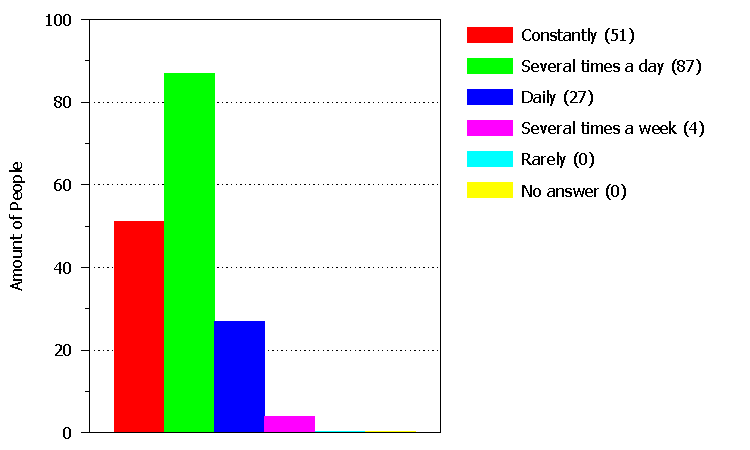
\includegraphics[width=1.0\textwidth]{201_Frequency_of_Internet_Usage.pdf}
\caption{Frequency of Internet usage}
\label{fig:internet_usage}
\end{figure}


\begin{figure}[hHtbp]
\centering
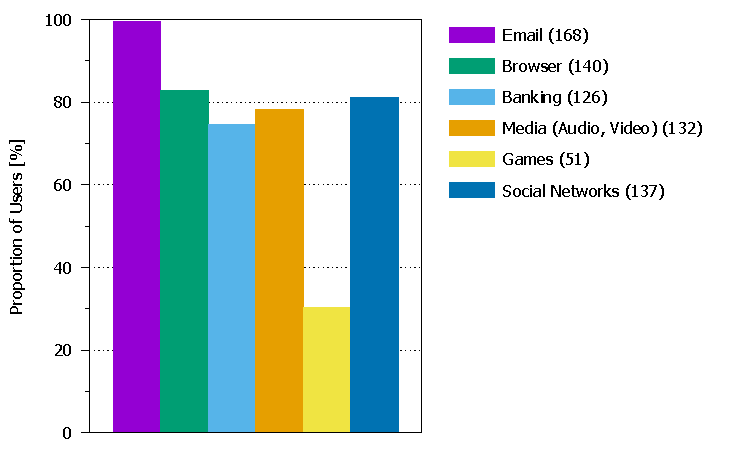
\includegraphics[width=1.0\textwidth]{202_Usage_Applications_Desktop.pdf}%
\caption{Usage of Internet applications on desktop computers}%
\label{fig:desktop_apps}%
\end{figure}

\begin{figure}[hHtbp]
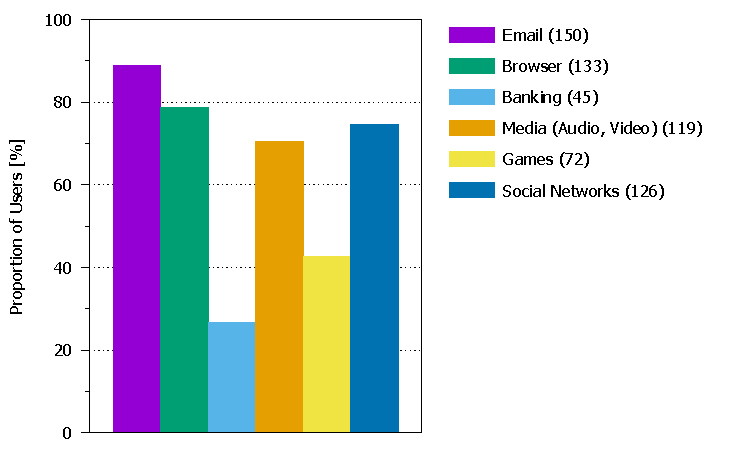
\includegraphics[width=1.0\textwidth]{204_Usage_Applications_Smartphone.pdf}%
\caption{Usage of Internet applications on smartphones}%
\label{fig:smartphone_apps}%
\end{figure}

\begin{figure}[hHtbp]
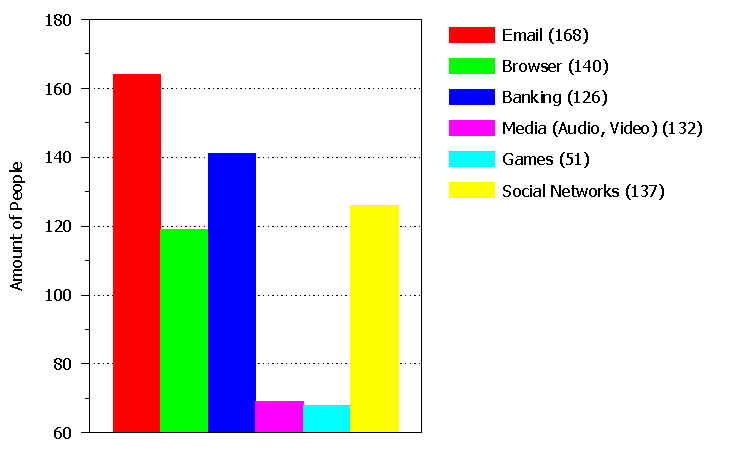
\includegraphics[width=1.0\textwidth]{401_Endangered_Services.pdf}%
\caption{Services endangered by phishing}%
\label{fig:endangered_services}%
\end{figure}

\begin{figure}[hHtbp]
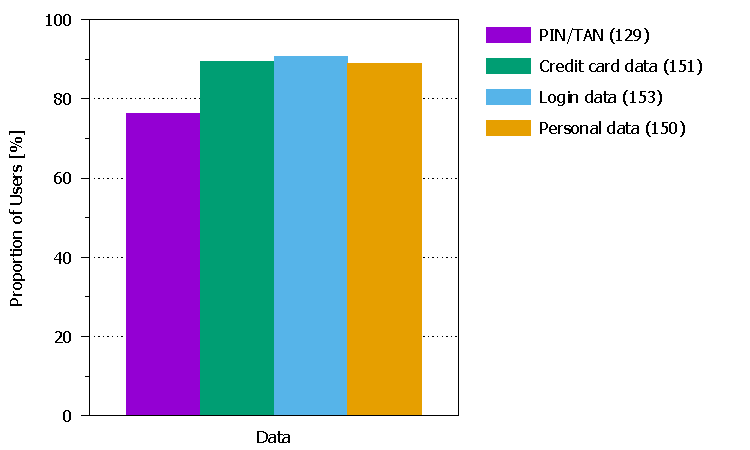
\includegraphics[width=1.0\textwidth]{402_Endangered_Data.pdf}%
\caption{Data endangered by phishing}%
\label{fig:endangered_data}%
\end{figure}
